\section{数据下载}
\subsection{安装下载工具}
\begin{frame}
    \frametitle{下载安装包}
    打开laadsOrderTool项目发布页面, 下载最新的安装包

    \url{https://github.com/xiaoke0O/LAADS-Order-Tool/releases}

    \begin{annotationimage}{width=\linewidth}{images/2B.1Release}
        \draw[red,very thick](0.24,0.58) rectangle (0.48,0.63);
    \end{annotationimage}
\end{frame}
\begin{frame}
    \frametitle{创建虚拟环境,以Conda为例}
    打开Conda 的命令窗口,输入以下命令并回车

    conda create -n run-laadsTool python=3.8 setuptools=52 -y
\end{frame}
\begin{frame}
    \frametitle{激活虚拟环境}
    输入激活命令,激活该新建的环境
    \begin{annotationimage}{width=\linewidth}{images/2B.2激活环境}
        \draw[red,very thick](0.23,0.38) rectangle (0.54,0.43);
        \draw[red,very thick](0.01,0.29) -- (0.16,0.29);
    \end{annotationimage}
\end{frame}
\begin{frame}
    \frametitle{使用pip 安装}

    继续在窗口输入pip install ,然后用鼠标将下载的安装包拖进来(就会自动输入安装包的
    路径),回车以安装
    \begin{annotationimage}{width=\linewidth}{images/2B.3安装}
        \draw[red,very thick](0.33,0.3) -- (0.96,0.3);
        \draw[red,very thick](0.01,0.25) -- (0.16,0.25);
    \end{annotationimage}
\end{frame}
\begin{frame}
    \frametitle{运行laadsOrderTool}
    安装成功后,继续输入laadsOrderTool,回车以运行
    \begin{annotationimage}{width=\linewidth}{images/2B.4运行}
        \draw[red,very thick](0.01,0.43) -- (0.24,0.43);
        \draw[red,very thick](0.33,0.12) -- (0.48,0.12);
    \end{annotationimage}
\end{frame}
\begin{frame}
    \frametitle{主界面}
    如果显示了了主界面,说明安装成功
    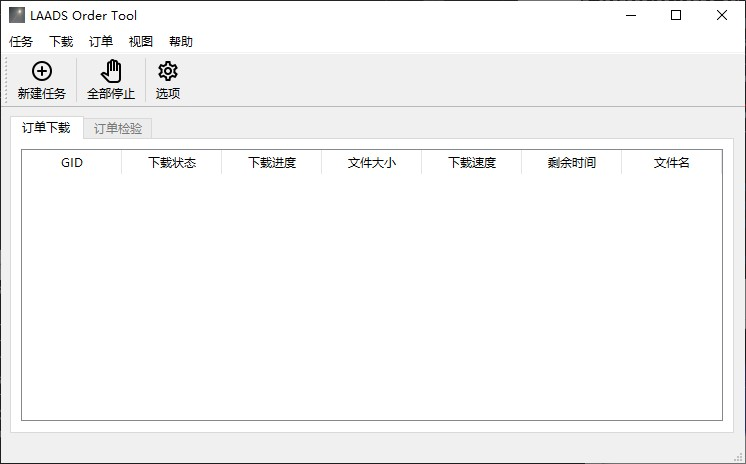
\includegraphics[width=\linewidth]{images/2B.5主界面.jpg}
\end{frame}
\subsection{获取授权Token}
\begin{frame}
    \frametitle{}
    在LAADS主页,点Profile,点击Generate Token
    \begin{annotationimage}{width=\linewidth}{images/8.登录完成}
        \draw[red,very thick](0.89,0.84) rectangle (0.98,0.88);
    \end{annotationimage}
\end{frame}

\begin{frame}
    \frametitle{复制Token}
    复制生成的Token
    \begin{annotationimage}{width=\linewidth}{images/2B.6Token}
        \draw[red,very thick](0.26,0.6) rectangle (0.71,0.72);
    \end{annotationimage}
\end{frame}
\begin{frame}
    \frametitle{设置laadsOrderTool}
    选择\underline{选项}按钮,在Token栏粘贴复制的Token,记得点OK
    \begin{annotationimage}{width=\linewidth}{images/2B.7设置Token}
        \draw[red,very thick](0.2,0.72) rectangle (0.25,0.88);
        \draw[red,very thick](0.34,0.62) rectangle (0.92,0.7);
        \draw[red,very thick](0.74,0.19) rectangle (0.84,0.26);
    \end{annotationimage}
\end{frame}
% --- 下载订单 ------------------------------------------------------------------
\subsection{导入订单下载}

\begin{frame}
    \frametitle{获取订单json链接}
    打开订单详情页,点击\underline{View as JSON}
    \begin{annotationimage}{width=\linewidth}{images/20.订单内容}
        \draw[red,very thick](0.58,0.74) rectangle (0.67,0.78);
    \end{annotationimage}
\end{frame}
\begin{frame}
    \frametitle{复制订单json地址}
    然后从浏览器地址栏复制订单的json地址
    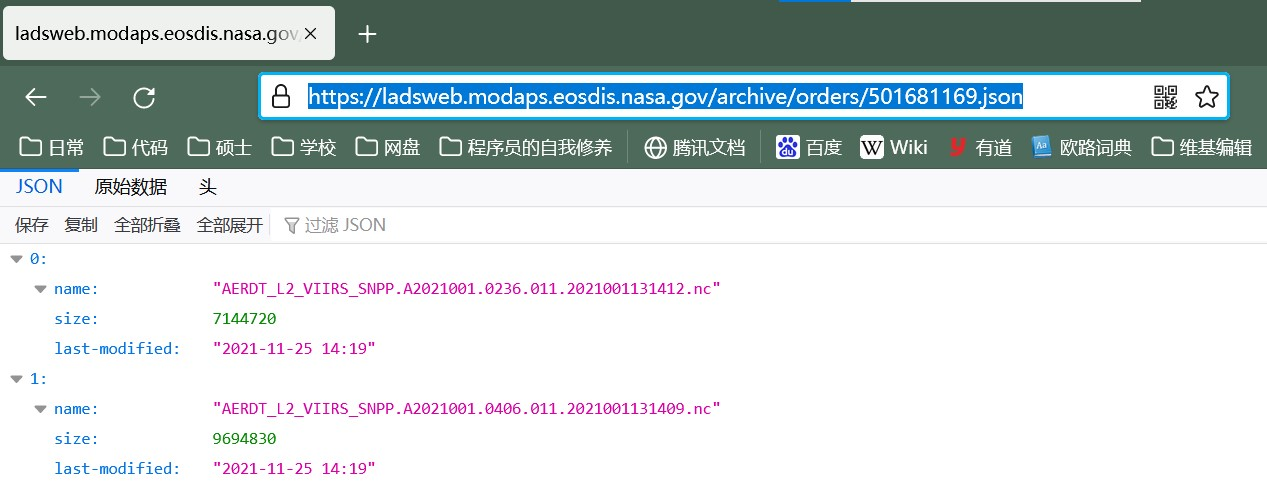
\includegraphics[width=\linewidth]{images/2B.8获取JSON.jpg}
\end{frame}
\begin{frame}
    \frametitle{新建任务}
    点击laadsOrderTool的\underline{新建任务},输入json地址,点击OK
    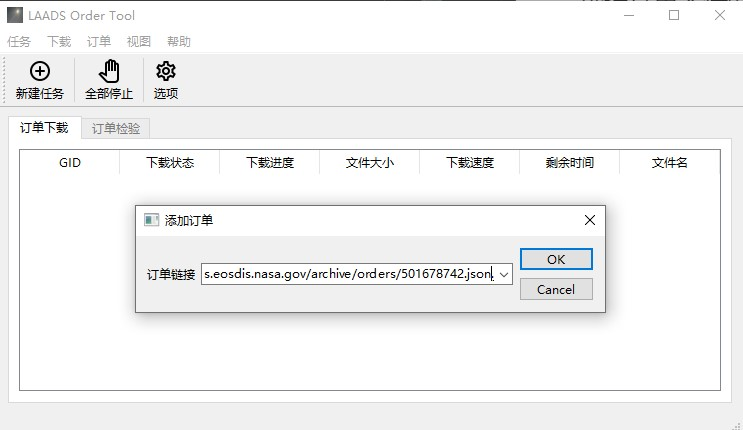
\includegraphics[width=\linewidth]{images/2B.9输入json}
\end{frame}

\begin{frame}
    \frametitle{选择下载文件}
    订单解析完成后,会显示出来文件条目。默认是全选。\\
    选择订单文件的存储位置,点击OK开始下载。
    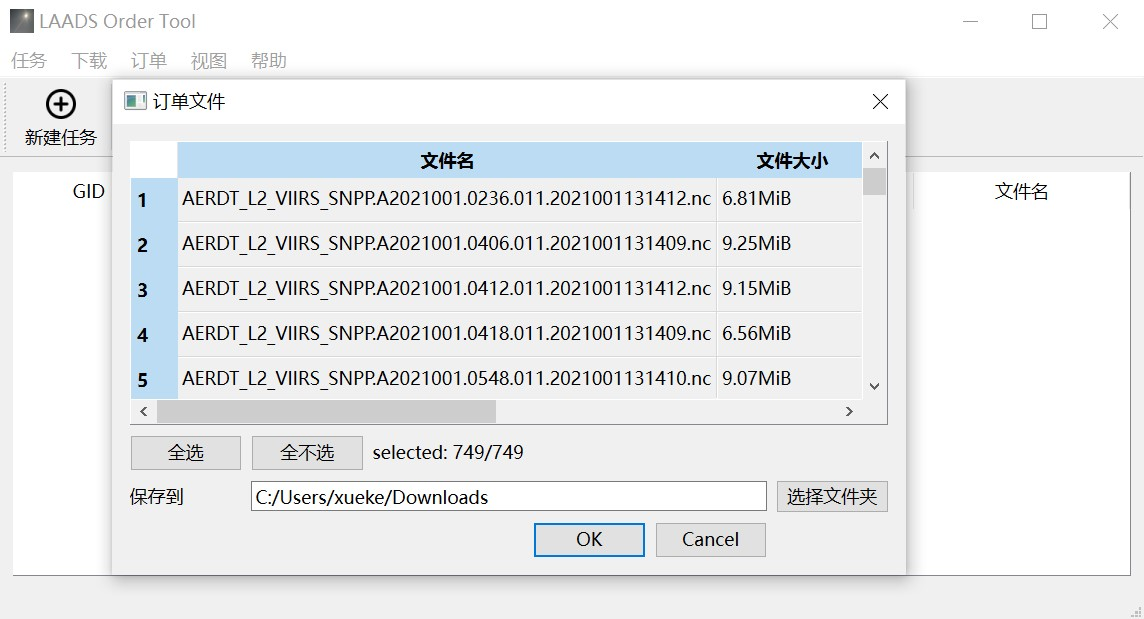
\includegraphics[width=\linewidth]{images/2B.10订单解析结果}
\end{frame}

\begin{frame}
    \frametitle{下载中}
    下载进行中,如果遇到速度为0的情况,如果网络没断,就耐心等待。
    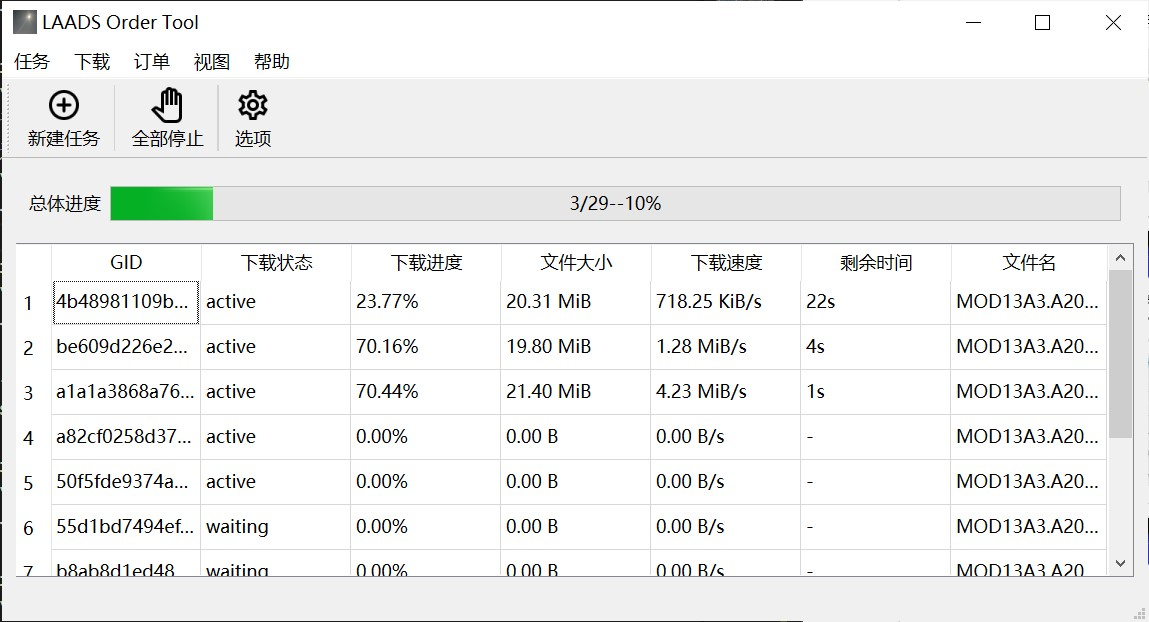
\includegraphics[width=\linewidth]{images/2B.11下载中.jpg}
\end{frame}

% --- 校验订单 ------------------------------------------------------------------
\subsection{自动校验订单}

\begin{frame}
    \frametitle{校验中}
    订单下载完成后会询问是否检查订单完整性的提示,强烈建议选择继续
    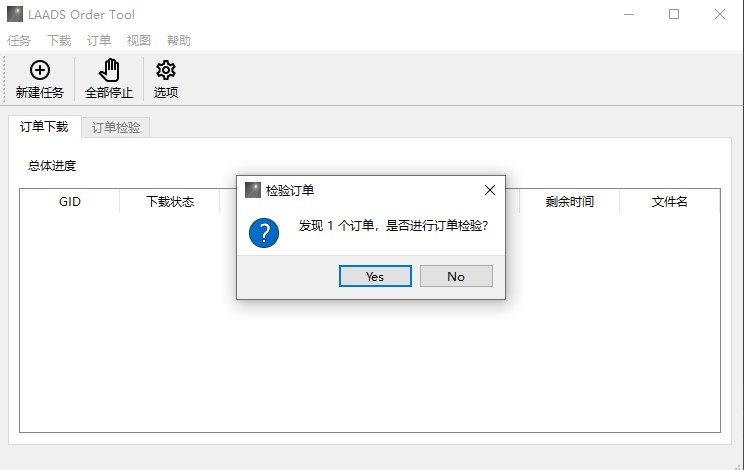
\includegraphics[width=\linewidth]{images/2B.12下载完成.jpg}
\end{frame}

\begin{frame}
    \frametitle{校验结果}
    检验结果展示
    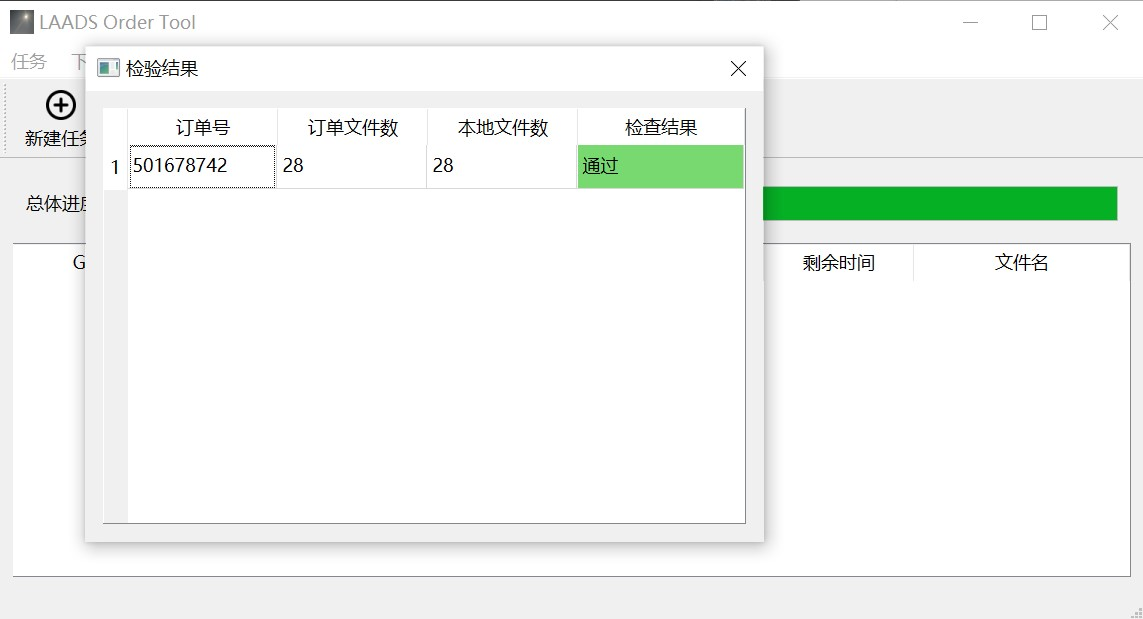
\includegraphics[width=\linewidth]{images/2B.13校验结果.jpg}
\end{frame}

\begin{frame}
    \frametitle{如果查出错误}
    如果有错误,检测结果就会标红,并且你可以点击红色区域,查看哪些文件出错了。
    \begin{columns}
        \column{.5\textwidth}
        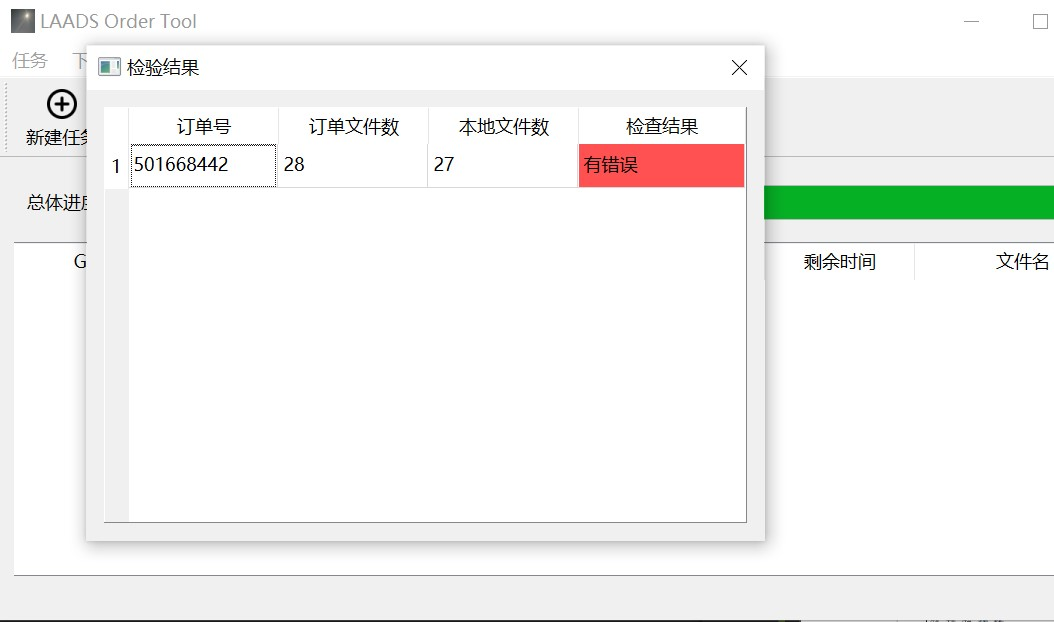
\includegraphics[width=\linewidth]{images/2B.14有错误.jpg}
        \column{.5\textwidth}
        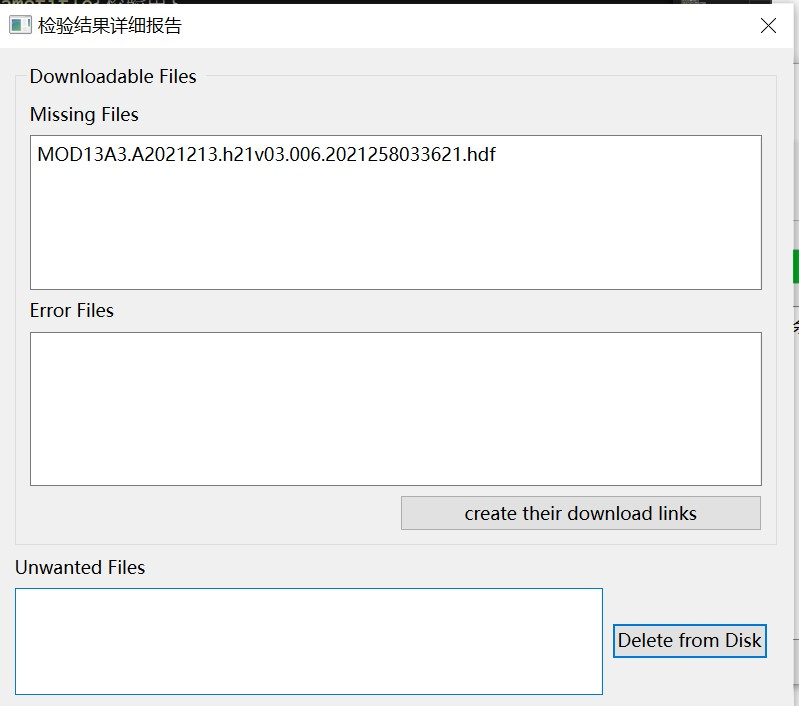
\includegraphics[width=\linewidth]{images/2B.15错误报告.jpg}
    \end{columns}
\end{frame}